\chapter{Matematikai függvények}
\thispagestyle{empty}

\section{Egyszerűbb matematikai függvények}

Az \textbf{ABS} függvény egy szám abszolút értékét
számítja ki. Tehát negatív argumentum esetén a függvény
eredménye pozitív. Például: ABS(-7)=7.

A \textbf{FACT} függvény kiszámítja egy szám
faktoriálisát. Definíció szerint 4!=1*2*3*4.

Az \textbf{INT} függvény a legközelebbi egészre kerekít le egy
számot. A negatív számok lefelé kerekítődnek a
legközelebbi egészre. Például: INT(5,6)=5 és  INT(-5,6)=-6.

Az \textbf{EVEN} függvény pozitív szám legközelebbi páros
egészre felkerekített értékét, illetve egy negatív szám
legközelebbi páros egészre lekerekített értékét adja
eredményül. Például: EVEN(4,6)=6 és  EVEN(-4,6) eredménye
-6.

Az \textbf{EXP} függvény. Az e-t a megadott hatványra emeli. Az e
állandó értéke megközelítőleg 2,71828. Az EXP(1)
eredménye maga az e szám.

A \textbf{GCD} függvény kiszámítja két vagy több egész
szám legnagyobb közös osztóját. A legnagyobb közös
osztó az a legnagyobb pozitív egész szám, amellyel maradék
nélkül osztható az összes megadott egész szám. Például:
a GCD(60;12;16) eredménye 4.

Az \textbf{LCM} függvény kiszámítja két vagy több szám
legkisebb közös többszörösét. Például LCM(18;30)
eredménye 90, mert ez a legkisebb szám, ami mind a 18-al, mind a
30-al maradék nélkül osztható.

Az \textbf{ISEVEN} függvény IGAZ értéket ad vissza, ha a szám
páros egész, HAMIS értéket, ha páratlan.

Az \textbf{ISODD} függvény IGAZ értéket ad vissza, ha a szám
páratlan, HAMIS értéket, ha a szám páros.

A \textbf{POWER} függvény hatványoz egy számot. Például a
POWER(12;2) eredménye egyenlő 12\^{}2, tehát 144.

A \textbf{PRODUCT} függvény összeszorozza az argumentumban
megadott számokat, eredményül a szorzatot adja.

A \textbf{MOD} függvény a maradékot adja eredményül egy
egész szám másik egész számmal való osztása után.
Például MOD(18;7) eredménye 4, mert a 18/7 osztás utáni
maradék 4.

A \textbf{ROUND} függvény egy szám meghatározott számú
tizedesjegyre kerekített értékét adja eredményül.
Például ROUND(4,155;2) eredménye 4,16 lesz. Fontos tudni, hogy a
cellaformátum módosításával is elérhetjük ugyanezt az
eredményt, de a cella valódi tartalma nem változik. Amikor
hivatkozunk rá, akkor az eredeti tartalmával fog számolni a Calc.

A \textbf{SQRT} függvény egy szám négyzetgyökét számítja
ki.

A \textbf{TRUNC} függvény levágja a szám tizedesjegyeit.
Például TRUNC(4,155;2) eredménye 4,15. A második argumentum nem
kötelező, elhagyva minden tizedesjegyet eldob: TRUNC(4,155) = 4.


\section{14. feladat}
{\itshape
Oldjuk meg, hogy az A1 cellába beírt, 1000-nél nem nagyobb
pozitív egész számról a PRÍM szöveg jelenjen meg az A2
cellában, ha a szám prímszám. Amennyiben a szám nem prím,
ugyanebben a cellában jelenjen meg az osztóinak a száma.}

{\itshape
Az A1 cella csak az 1, 2, {\dots}, 1000 tartományból fogadjon
értékeket.}

A prím számok csak eggyel és önmagukkal
oszthatók maradék nélkül. A feladat tehát az, hogy
megállapítsuk egy számról, két osztója van. A definíció
szerint az 1-et nem soroljuk a prím számok közé.

A calc03 munkafüzet második munkalapját nevezzük át
,,prím''-re. Írjunk egy
tetszőleges, 1000-nél kisebb egész számot az A1 cellába. A
B oszlopban hozzunk létre számoszlopot 1000-ig a 10. feladatban
tárgyalt módon. A C oszlopban pedig számítsuk ki az A1
cellába írt szám és a B oszlop megfelelő elemének
hányadosát (\ref{14-feladat} ábra).

\begin{figure}[!h]
\begin{center}
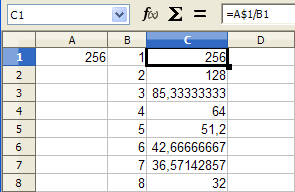
\includegraphics[width=7.203cm]{oocalcv1-img77.png}
\caption{14. feladat}\label{14-feladat}
\end{center}
\end{figure}

A C oszlopban mind az 1000 értéket kiszámíthatjuk, ha kettőt
kattintunk a cella jobb alsó részében megjelenő
célkereszttel. Ilyenkor a Calc másolja a képletet míg a B
oszlopban kitöltött cellákat talál.

Kaptunk egy számoszlopot, amely egész számokból és tizedes
törtekből áll. Az egész számok darabszáma megadja az
osztók számát. Ahhoz, hogy ezt meghatározzuk, a D oszlopban
számítsuk ki a C oszlop értékeinek egész részét a TRUNC
függvényt használva. Az E oszlopban pedig az IF függvényt
felhasználva jelenítsünk meg 1-et, ha a tőle balra lévő
két cella tartalma egyenlő, ellenkező esetben pedig nullát.
(\ref{14-feladatIF} ábra).

\begin{figure}[!h]
\begin{center}
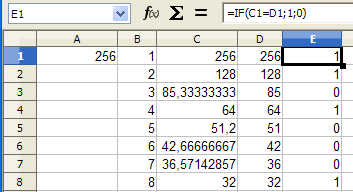
\includegraphics[width=9.338cm]{oocalcv1-img78.png}
\caption{14. feladat -- IF}\label{14-feladatIF}
\end{center}
\end{figure}

Az E oszlop összege megadja az A1-be írt szám osztóinak a
számát. Az F1 cellában a SUM függvénnyel számítsuk ezt
ki. Az IF függvénnyel jelenítsük meg a PRÍM szöveget, ha az
osztók száma kettő (\ref{14-feladatPrím} ábra).

\begin{figure}[!h]
\begin{center}
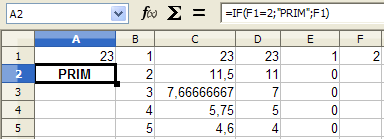
\includegraphics[width=9.158cm]{oocalcv1-img79.png}
\caption{14. feladat -- PRÍM}\label{14-feladatPrím}
\end{center}
\end{figure}

Az A3 cellában megjeleníthetjük az ,,osztója
van'' szöveget is, abban az esetben, ha nem prím
számot írunk az A1 cellába. Prím szám esetén a cella üres
marad (\ref{14-feladatOsztó} ábra).

\begin{figure}[!h]
\begin{center}
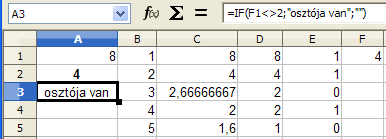
\includegraphics[width=9.211cm]{oocalcv1-img80.png}
\caption{14. feladat -- Van osztója}\label{14-feladatOsztó}
\end{center}
\end{figure}

A MOD és a COUNTIF függvények segítségével egyszerűbben
is megoldható a feladat. Ezt  végezzük el önállóan!

\begin{figure}[!h]
\begin{center}
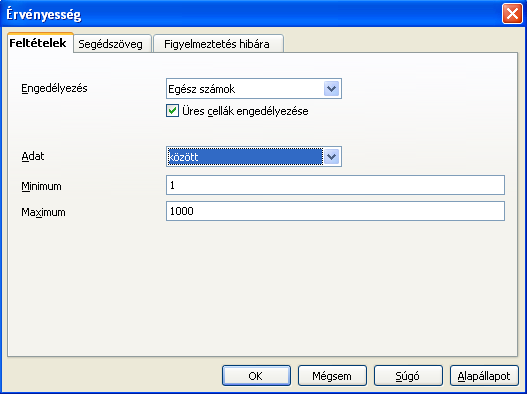
\includegraphics[width=11.444cm]{oocalcv1-img81.png}
\caption{14. feladat -- Érvényesség, feltételek}\label{14-feladatFeltétel}
\end{center}
\end{figure}

\begin{figure}[!h ]
\begin{center}
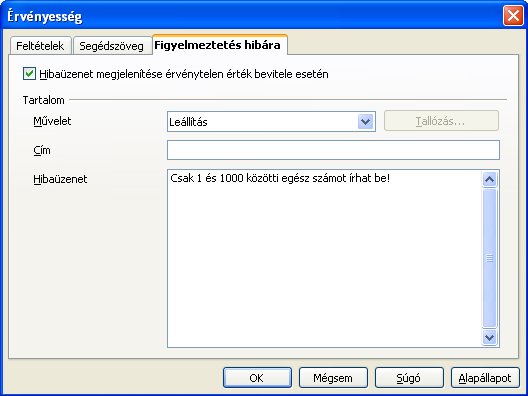
\includegraphics[width=11.47cm]{oocalcv1-img82.png}
\caption{14. feladat -- Érvényesség, figyelmeztetés}\label{14-feladatFigy}
\end{center}
\end{figure}

Ezernél nagyobb számot írva az A1 cellába hibás eredményt
kaphatunk. A Calcban egyszerűen megoldható, hogy cellába csak a
megadott tartományból írhassunk be számot. Ehhez válasszuk az
\textbf{Adatok} menüpont \textbf{Érvényesség} parancsát.
Állítsuk be \aref{14-feladatFeltétel} ábrán látható értékeket.

Kapcsoljuk be a hibaüzenet megjelenítését és a
\textbf{Művelet}-ek közül válasszuk a
\textbf{Leállítás}t (\ref{14-feladatFigy} ábra).  

A \textbf{Hibaüzenet} szövegét megadva az fog megjelenni nem
megfelelő tartalom beírása esetén (\ref{14-feladatHiba} ábra).

\begin{figure}[!h]
\begin{center}
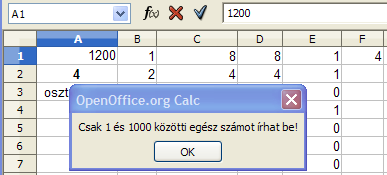
\includegraphics[width=9.238cm]{oocalcv1-img83.png}
\caption{14.  feladat -- Hibaüzenet}\label{14-feladatHiba}
\end{center}
\end{figure}


\section{15. feladat}
{\itshape
Az A2 és a A3 cellákba írt pozitív egész számokból
kialakított törtet egyszerűsítsük a legnagyobb közös
osztóval. Amennyiben a kapott tört áltört, azt alakítsuk át
vegyes törtté. Ebben az esetben a D1 cellában jelenjen meg az
,,Áltört'' szöveg. Amennyiben A2
és az A3 hányadosa egész szám, azt is számítsuk ki, és a
D1 cellában jelenjen meg az
,,Egész'' szöveg.}

A calc03 munkafüzet harmadik munkalapját nevezzük át tört-re.
Az A2 cellába írjunk hatot, az A3  cellába négyet. Amikor a
két szám legnagyobb közös osztója eggyel egyenlő,
,,A tört nem
egyszerűsíthető'' szöveg jelenik meg az
A5 cellában. Ellenkező esetben az ,,A tört
egyszerűsíthető'' szöveg (\ref{15-feladat} ábra),
valamint D5 cellában megjelenik a GCD függvény eredménye is.

A D5 tartalma:
{\sffamily\bfseries{=IF(GCD(A2;A3)<>1;GCD(A2;A3);"")}}.

\begin{figure}[!h]
\begin{center}
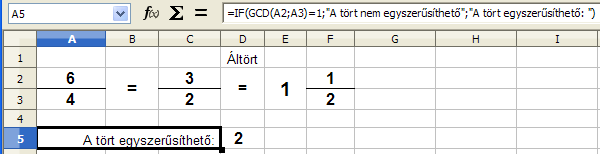
\includegraphics[width=13.873cm]{oocalcv1-img84.png}
\caption{15. feladat}\label{15-feladat}
\end{center}
\end{figure}

Amikor az egyszerűsített tört számlálója nagyobb mint a
nevezője, a D1 cella az ,,Áltört'' szöveget mutatja. Az
,,egész'' szöveg jelenik meg, ha a nevező értéke 1, valódi
tört esetén pedig üres marad.  \Aref{15-feladatIFek} ábrán
látjuk, hogy ezt két egymásba ágyazott IF
függvénnyel egyszerűen megoldhatjuk.

\begin{figure}[!h]
\begin{center}
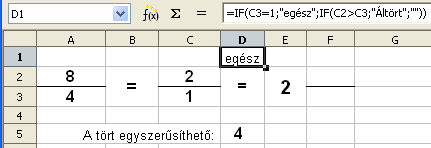
\includegraphics[width=10.404cm]{oocalcv1-img85.png}
\caption{15. feladat -- Egymásba ágyazott IF-ek}\label{15-feladatIFek}
\end{center}
\end{figure}

Valódi tört beírásakor a D2 cellában az egyenlőség jele
sem jelenik meg (\ref{15-feladatValódi} ábra).

\begin{figure}[!h]
\begin{center}
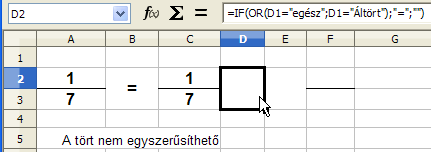
\includegraphics[width=10.402cm]{oocalcv1-img86.png}
\caption{15. feladat -- Valódi tört}\label{15-feladatValódi}
\end{center}
\end{figure}

Az E2 cella tartalma csak akkor számítódik ki, ha a D2
egyenlőségjelet tartalmaz.

Az E2 tartalma:
{\sffamily\bfseries{=IF(D2="=";TRUNC(C2/C3);"")}}.

Az F2 és az F3 pedig csak áltört esetén:

Az F2 cella tartalma:
{\sffamily\bfseries{=IF(D1="Áltört";C2-E2*F3;"")}}.

Az F3 cella tartalma:
{\sffamily\bfseries{=IF(D1="Áltört";C3;"")}}.


\section{Logaritmusfüggvények}

Az \textbf{LN} függvény kiszámítja egy szám
,,$e$'' állandón alapuló
természetes logaritmusát. Az $e$ állandó értéke
megközelítőleg 2,71828182845904.

\noindent A \textbf{LOG} függvény szám megadott alapú logaritmusát adja
eredményül. Szintaxisa: LOG(szám;alap)

\noindent A \textbf{LOG10} függvény kiszámítja a szám tízes alapú
logaritmusát.


\section{16. feladat}
{\itshape
Számítsuk ki az A2:A76 tartományba létrehozott 0,1, 0,2,
{\ldots}, 7,5 értékeknél a következő függvények
eredményeit:  $\log_{2}(x),\ln(x),\log_{10}(x),\log_{0,5}(x)$
Építsük meg a függvények grafikonjait.}

Az A2:A76 tartomány számadatainak létrehozásához írjuk be az
első két értéket, ezeket kijelölve és lefelé másolva
(\ref{16-feladat} ábra) a Calc kitölti a tartományt.

\begin{figure}[!h]
\begin{center}
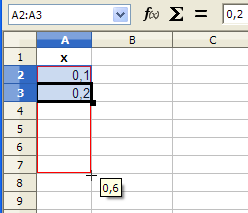
\includegraphics[width=6.56cm]{oocalcv1-img87.png}
\caption{16. feladat}\label{16-feladat}
\end{center}
\end{figure}

\begin{figure}[!h]
\begin{center}
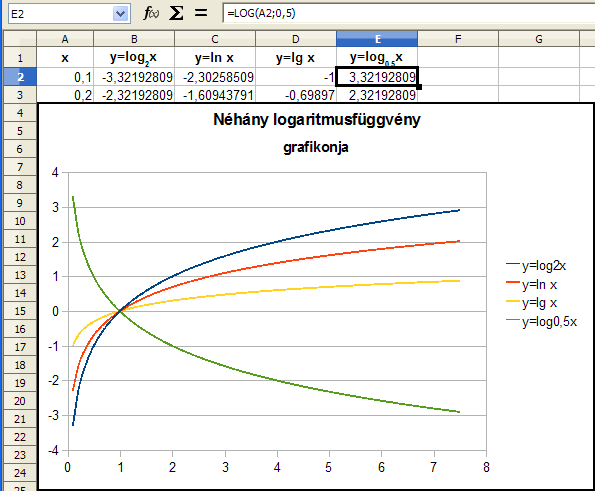
\includegraphics[width=14.739cm]{oocalcv1-img88.png}
\caption{16. feladat --  grafikon}\label{16-feladatGrafikon}
\end{center}
\end{figure}

A B1, C1, D1 és E1 cellákba írjuk a függvények neveit és
számítsuk ki az értékeket. A diagramtündér
segítségével könnyen elkészíthetjük a diagramot,
 előzőleg kijelölve az A2:E76 tartományt (\ref{16-feladatGrafikon} ábra).

\section{Trigonometrikus függvények}

A Calc beépített függvényei között megtaláljuk a
trigonometrikus függvényeket és azok inverzeit is. A fontosabb
trigonometrikus, valamint azokkal kapcsolatos függvényeket
\aref{TrigFüggvények} táblázat mutatja.

\begin{table}
\begin{center}
\caption{A legfontosabb trigonometrikus függvények}\label{TrigFüggvények}
\begin{tabular}{|m{2.5cm}|m{8cm}|}
\hline
SIN &
 kiszámítja egy adott szög (radiánban) szinuszát.\\ \hline
COS &
 kiszámítja egy adott szög (radiánban) koszinuszát.\\ \hline
SINH &
 kiszámítja egy szám szinusz hiperbolikuszát.\\ \hline
COSH &
 kiszámítja egy szám koszinusz hiperbolikuszát.\\ \hline
TAN &
 kiszámítja egy adott szög (radiánban) tangensét.\\ \hline
TANH &
 kiszámítja egy szám tangens hiperbolikuszát.\\ \hline
PI &
 A ${\pi}$ matematikai állandó 14 tizedesjegyre kerekített
értékét adja vissza, ami 3,14159265358979.\\ \hline
RADIANS &
átszámítja a fok értéket radiánra.\\ \hline
\end{tabular}
\end{center}
\end{table}


\clearpage
\section{17. feladat}

{\itshape
Ábrázoljuk Pont(XY) diagramon a  $y=a\ast \sin (c\ast
(b+\mathit{{\alpha}}))$ függvény grafikonját a [-360; +360]
intervallumon.  Az a, b és c értékeket a E1, H1 és K1 cellák
tartalmazzák.}

Az A2:A74 tartományban hozzuk létre az ${\alpha}$ értékeket. A
függvény értékeinek kiszámításánál a megfelelő
cellahivatkozásoknál használjunk abszolút cellacímzést,
és ne feledjük, hogy a fokértékeket át kell alakítani
radiánra (\ref{17-feladatGrafikon} ábra).

\begin{figure}[!h]
\begin{center}
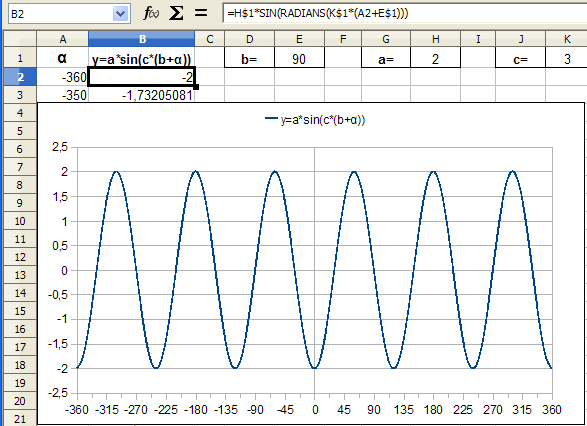
\includegraphics[width=15.529cm]{oocalcv1-img89.png}
\caption{17. feladat --  grafikon}\label{17-feladatGrafikon}
\end{center}
\end{figure}

Az ebben a fejezetben tárgyalt függvényeket \aref{8-fejezetFüggvények}
táblázatban találjuk meg.

\begin{table}[!h]
\begin{center}
\caption{A fejezetben tárgyalt függvények}\label{8-fejezetFüggvények}
\begin{tabular}{|m{2.5cm}|m{8cm}|m{3cm}|}
\hline
 & & \multicolumn{1}{c|}{\textbf{Megfelelője a}} \\
\multicolumn{1}{|c|}{\textbf{A függvény}}&
\multicolumn{1}{c|}{\textbf{Funkciója}}&
\multicolumn{1}{c|}{\textbf{magyar}} \\
\multicolumn{1}{|c|}{\textbf{neve}} & &
\multicolumn{1}{c|}{\textbf{Microsoft}} \\
 & & \multicolumn{1}{c|}{\textbf{Excelben}} \\
\hline
ABS & Egy szám abszolút értékét számítja ki. & ABS\\ \hline
FACT & Egy szám faktoriálisát számítja ki. & FAKT\\ \hline
INT & A legközelebbi egészre kerekít  egy számot. & INT\\ \hline
EVEN & A legközelebbi páros egészre kerekít. & PÁROS\\ \hline
EXP & Az e-t a megadott hatványra emeli. & KITEV\H{O}\\ \hline
GCD & Legnagyobb közös osztó kiszámítása. & GCD\\ \hline
LCM & Legkisebb közös többszörös kiszámítása. & LCM\\ \hline
ISEVEN & Igaz értéket ad vissza, ha a szám páros. & ISEVEN\\ \hline
ISODD & Igaz értéket ad vissza, ha a szám páratlan. & ISODD\\ \hline
POWER & Hatványoz egy számot. & HATVÁNY\\ \hline
PRODUCT & Összeszorozza az argumentumban megadott számokat. & SZORZAT\\ \hline
MOD & Osztási maradékot jeleníti meg. & MOD\\ \hline
ROUND & Meghatározott számú tizedesjegyre kerekít. & KEREK\\ \hline
SQRT & Egy szám négyzetgyökét számítja ki. & GYÖK\\ \hline
TRUNC & Levágja a szám tizedesjegyeit. & CSONK\\ \hline
LN & Természetes logaritmust számol. & LN\\ \hline
LOG & Megadott alapú logaritmust számol. & LOG\\ \hline
LOG10 & Tízes alapú logaritmust számol. & LOG10\\ \hline
SIN & Egy adott szög szinuszát számítja ki. & SIN\\ \hline
COS & Egy adott szög koszinuszát számítja ki. & COS\\ \hline
SINH & Egy szám koszinusz hiperbolikuszát számítja ki. & SINH\\ \hline
COSH & Egy szám koszinusz hiperbolikuszát számítja ki. & COSH\\ \hline
TAN & Egy szög tangensét számítja ki. & TAN\\ \hline
TANH & Egy szám tangens  hiperbolikuszát számítja ki. & TANH\\ \hline
PI & A PI matematikai állandót adja meg. & PI\\ \hline
RADIANS & Fokot, radiánná alakít. & RADIÁN\\ \hline
\end{tabular}
\end{center}
\end{table}

